\section{Sprint 7}

\subsection*{Summary}

\begin{table}[H]
	\centering
	\begin{tabular}{ll}
		\toprule
		\multicolumn{2}{c}{\textbf{Sprint 7}}\\
		\midrule
		\textbf{Periode} & 11.05.2015 12:00 Uhr\textendash 26.05.2015 12:00 Uhr\\
		\textbf{Stunden Soll} & \SI{144}{\hour}\\
		\textbf{Stunden Plan} & \SI{147}{\hour} \\
		\textbf{Stunden Ist} & \SI{146.8}{\hour}\\
		\bottomrule
	\end{tabular}
\end{table}

\begin{figure}[H]
	\centering
	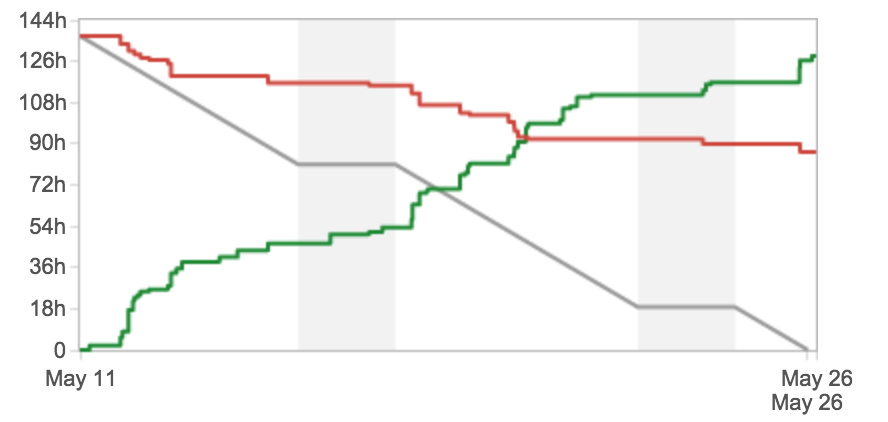
\includegraphics{fig/bd-sprint-7}
	\label{fig:pm:bd-sprint-7}
	\caption*{Burndown Chart Sprint 7}
\end{figure}

\subsection*{Ziele}
Die Kernfunktionalität von \acf{odh} steht und die Use-Cases wurden weitestgehend umgesetzt. Somit ist dieser Sprint als reiner Bugfixing oder Improvement/Enhancement Sprint gedacht. Vor allem im Bereich mit Geo-Daten sind noch einige Fehlersituationen denkbar.

\subsection*{Abgeschlossen}
Folgende High-level (ohne Subtasks) Jira Tasks wurden während Sprint 7 abgeschlossen. 

\begin{table}[H]	
\centering
\begin{tabular}{ll}
\toprule
\textbf{JIRA-Key} & \textbf{Summary}\\
\midrule
DAT-139 & Bugfixing \\
DAT-141 & UI Tests \\
DAT-143 & Update \& Delete Package ("Documents") \\
DAT-148 & Organisation, Planung \& Kommunikation Sprint 7 \\
DAT-149 & Projektmeetings Sprint 7 \\
DAT-150 & Übrige Aufwände Sprint 7 \\
DAT-151 & Screencast erstellen \\
DAT-152 & Logo erstellen \\
DAT-175 & Interlis-Modell verwenden für Interlis-Konvertierung \\
DAT-176 & Expressions in Join-Conditions implementieren \\
\bottomrule
\end{tabular}	
\end{table}

\subsection*{Probleme}
Im letzten Sprint wurde aufgrund der fehlenden GeoPackage-Kompatibilität auf GDAL 1.11.1 gewechselt. In diesem Sprint sahen wir uns nach Experimenten mit diversen Versionen inkl. 2.0.0beta1 gezwungen, wieder auf GDAL 1.10.1 zu wechseln.